\documentclass[]{book}
\usepackage{lmodern}
\usepackage{amssymb,amsmath}
\usepackage{ifxetex,ifluatex}
\usepackage{fixltx2e} % provides \textsubscript
\ifnum 0\ifxetex 1\fi\ifluatex 1\fi=0 % if pdftex
  \usepackage[T1]{fontenc}
  \usepackage[utf8]{inputenc}
\else % if luatex or xelatex
  \ifxetex
    \usepackage{mathspec}
  \else
    \usepackage{fontspec}
  \fi
  \defaultfontfeatures{Ligatures=TeX,Scale=MatchLowercase}
\fi
% use upquote if available, for straight quotes in verbatim environments
\IfFileExists{upquote.sty}{\usepackage{upquote}}{}
% use microtype if available
\IfFileExists{microtype.sty}{%
\usepackage{microtype}
\UseMicrotypeSet[protrusion]{basicmath} % disable protrusion for tt fonts
}{}
\usepackage[margin=1in]{geometry}
\usepackage{hyperref}
\hypersetup{unicode=true,
            pdftitle={Your first date with R},
            pdfauthor={Quantide},
            pdfborder={0 0 0},
            breaklinks=true}
\urlstyle{same}  % don't use monospace font for urls
\usepackage{natbib}
\bibliographystyle{plainnat}
\usepackage{color}
\usepackage{fancyvrb}
\newcommand{\VerbBar}{|}
\newcommand{\VERB}{\Verb[commandchars=\\\{\}]}
\DefineVerbatimEnvironment{Highlighting}{Verbatim}{commandchars=\\\{\}}
% Add ',fontsize=\small' for more characters per line
\usepackage{framed}
\definecolor{shadecolor}{RGB}{248,248,248}
\newenvironment{Shaded}{\begin{snugshade}}{\end{snugshade}}
\newcommand{\KeywordTok}[1]{\textcolor[rgb]{0.13,0.29,0.53}{\textbf{{#1}}}}
\newcommand{\DataTypeTok}[1]{\textcolor[rgb]{0.13,0.29,0.53}{{#1}}}
\newcommand{\DecValTok}[1]{\textcolor[rgb]{0.00,0.00,0.81}{{#1}}}
\newcommand{\BaseNTok}[1]{\textcolor[rgb]{0.00,0.00,0.81}{{#1}}}
\newcommand{\FloatTok}[1]{\textcolor[rgb]{0.00,0.00,0.81}{{#1}}}
\newcommand{\ConstantTok}[1]{\textcolor[rgb]{0.00,0.00,0.00}{{#1}}}
\newcommand{\CharTok}[1]{\textcolor[rgb]{0.31,0.60,0.02}{{#1}}}
\newcommand{\SpecialCharTok}[1]{\textcolor[rgb]{0.00,0.00,0.00}{{#1}}}
\newcommand{\StringTok}[1]{\textcolor[rgb]{0.31,0.60,0.02}{{#1}}}
\newcommand{\VerbatimStringTok}[1]{\textcolor[rgb]{0.31,0.60,0.02}{{#1}}}
\newcommand{\SpecialStringTok}[1]{\textcolor[rgb]{0.31,0.60,0.02}{{#1}}}
\newcommand{\ImportTok}[1]{{#1}}
\newcommand{\CommentTok}[1]{\textcolor[rgb]{0.56,0.35,0.01}{\textit{{#1}}}}
\newcommand{\DocumentationTok}[1]{\textcolor[rgb]{0.56,0.35,0.01}{\textbf{\textit{{#1}}}}}
\newcommand{\AnnotationTok}[1]{\textcolor[rgb]{0.56,0.35,0.01}{\textbf{\textit{{#1}}}}}
\newcommand{\CommentVarTok}[1]{\textcolor[rgb]{0.56,0.35,0.01}{\textbf{\textit{{#1}}}}}
\newcommand{\OtherTok}[1]{\textcolor[rgb]{0.56,0.35,0.01}{{#1}}}
\newcommand{\FunctionTok}[1]{\textcolor[rgb]{0.00,0.00,0.00}{{#1}}}
\newcommand{\VariableTok}[1]{\textcolor[rgb]{0.00,0.00,0.00}{{#1}}}
\newcommand{\ControlFlowTok}[1]{\textcolor[rgb]{0.13,0.29,0.53}{\textbf{{#1}}}}
\newcommand{\OperatorTok}[1]{\textcolor[rgb]{0.81,0.36,0.00}{\textbf{{#1}}}}
\newcommand{\BuiltInTok}[1]{{#1}}
\newcommand{\ExtensionTok}[1]{{#1}}
\newcommand{\PreprocessorTok}[1]{\textcolor[rgb]{0.56,0.35,0.01}{\textit{{#1}}}}
\newcommand{\AttributeTok}[1]{\textcolor[rgb]{0.77,0.63,0.00}{{#1}}}
\newcommand{\RegionMarkerTok}[1]{{#1}}
\newcommand{\InformationTok}[1]{\textcolor[rgb]{0.56,0.35,0.01}{\textbf{\textit{{#1}}}}}
\newcommand{\WarningTok}[1]{\textcolor[rgb]{0.56,0.35,0.01}{\textbf{\textit{{#1}}}}}
\newcommand{\AlertTok}[1]{\textcolor[rgb]{0.94,0.16,0.16}{{#1}}}
\newcommand{\ErrorTok}[1]{\textcolor[rgb]{0.64,0.00,0.00}{\textbf{{#1}}}}
\newcommand{\NormalTok}[1]{{#1}}
\usepackage{longtable,booktabs}
\usepackage{graphicx,grffile}
\makeatletter
\def\maxwidth{\ifdim\Gin@nat@width>\linewidth\linewidth\else\Gin@nat@width\fi}
\def\maxheight{\ifdim\Gin@nat@height>\textheight\textheight\else\Gin@nat@height\fi}
\makeatother
% Scale images if necessary, so that they will not overflow the page
% margins by default, and it is still possible to overwrite the defaults
% using explicit options in \includegraphics[width, height, ...]{}
\setkeys{Gin}{width=\maxwidth,height=\maxheight,keepaspectratio}
\IfFileExists{parskip.sty}{%
\usepackage{parskip}
}{% else
\setlength{\parindent}{0pt}
\setlength{\parskip}{6pt plus 2pt minus 1pt}
}
\setlength{\emergencystretch}{3em}  % prevent overfull lines
\providecommand{\tightlist}{%
  \setlength{\itemsep}{0pt}\setlength{\parskip}{0pt}}
\setcounter{secnumdepth}{5}
% Redefines (sub)paragraphs to behave more like sections
\ifx\paragraph\undefined\else
\let\oldparagraph\paragraph
\renewcommand{\paragraph}[1]{\oldparagraph{#1}\mbox{}}
\fi
\ifx\subparagraph\undefined\else
\let\oldsubparagraph\subparagraph
\renewcommand{\subparagraph}[1]{\oldsubparagraph{#1}\mbox{}}
\fi

%%% Use protect on footnotes to avoid problems with footnotes in titles
\let\rmarkdownfootnote\footnote%
\def\footnote{\protect\rmarkdownfootnote}

%%% Change title format to be more compact
\usepackage{titling}

% Create subtitle command for use in maketitle
\newcommand{\subtitle}[1]{
  \posttitle{
    \begin{center}\large#1\end{center}
    }
}

\setlength{\droptitle}{-2em}
  \title{Your first date with R}
  \pretitle{\vspace{\droptitle}\centering\huge}
  \posttitle{\par}
\subtitle{Exercise Book}
  \author{Quantide}
  \preauthor{\centering\large\emph}
  \postauthor{\par}
  \predate{\centering\large\emph}
  \postdate{\par}
  \date{2017-01-20}

\usepackage{booktabs}

\def\tightlist{}



%----------------------------------------------------------------%
%                          COPERTINA                             %
%----------------------------------------------------------------%

\makeatletter

\def\thickhrulefill{\leavevmode \leaders \hrule height 1pt\hfill \kern \z@}

\def\maketitle{%
  \null
  \thispagestyle{empty}%
  % scommentare se si vuole costruire l'eserciziario ( commentare la riga dopo)
  % \begin{flushleft}
\includegraphics[scale=.175]{exercises/images/quantide.png}\end{flushleft}
  %\hspace{-2cm}
   \begin{flushleft}
\includegraphics[width=50mm]{./images/logo-microsoft.png}\end{flushleft}
  \vspace{-2cm}
  % scommentare se si vuole costruire l'eserciziario ( commentare la riga dopo)
  % \begin{flushright}
\includegraphics[scale=.25]{exercises/images/R-training.png}\end{flushright}
  \begin{flushright}
\includegraphics[width=50mm]{./images/quantide.png}\end{flushright}
  \vskip 5cm
  \hrule height 2pt
  \begin{center} \par \huge \strut \textbf{$My  First  Date  with  R$}\\ $Exercise  Book$ \par  \end{center}
  \vspace{0.5cm}
  \hrule height 2pt
  \vspace{0.5cm}
  
\includegraphics[width=165mm]{./images/locandina.png}
  \clearpage
}

\makeatother
%----------------------------------------------------------------%

\begin{document}
\maketitle

{
\setcounter{tocdepth}{1}
\tableofcontents
}
\chapter{Introduction}\label{introduction}

In this document you will find some exercises about these sections:

\begin{itemize}
\tightlist
\item
  \emph{Your First R session}
\item
  \emph{Data Objects}
\item
  \emph{Data Import from external sources}
\item
  \emph{Data Manipulation with R}
\item
  \emph{Data Discovery with R}
\item
  \emph{Data Visualization with R}
\item
  \emph{Statistical Models with R}
\item
  \emph{Data Mining with R}
\end{itemize}

\chapter{Your first R session}\label{your-first-r-session}

\section{Aritmetic with R}\label{aritmetic-with-r}

\subsection{Exercise 1}\label{exercise-1}

Calculate your body mass index dividing your body mass (kg) by the
square of your body height (m) (\(kg/m^2\))

\section{Assignment}\label{assignment}

\subsection{Exercise 1}\label{exercise-1-1}

\begin{enumerate}
\def\labelenumi{\alph{enumi}.}
\item
  Assign your age (in number) to \texttt{age} variable.
\item
  Print out the value of the variable \texttt{age}.
\item
  Remove the variable \texttt{age} from the workspace, by using
  \texttt{rm()} function.
\end{enumerate}

\subsection{Exercise 2}\label{exercise-2}

Suppose you want to buy 10 roses and 8 sunflowers in a flower shop. The
roses cost 3 euros each and the sunflowers 2 euros each.

\begin{enumerate}
\def\labelenumi{\alph{enumi}.}
\item
  Assign the total cost of roses to \texttt{roses\_cost} variable and
  the total cost of sunflowers to \texttt{sunflowers\_cost} variable.
\item
  Calculate the total cost of flowers by adding \texttt{roses\_cost} and
  \texttt{sunflowers\_cost} variables and assign it to
  \texttt{flowers\_cost} variable.
\item
  Print out the value of the variable \texttt{flowers\_cost}.
\item
  List the objects in the current R session, by using \texttt{ls()}
  function.
\end{enumerate}

\chapter{Data Objects}\label{data-objects}

\section{Data Frames, Vectors and
Factors}\label{data-frames-vectors-and-factors}

\subsection{Exercise 1}\label{exercise-1-2}

\begin{enumerate}
\def\labelenumi{\alph{enumi}.}
\tightlist
\item
  Generate a data frame, named \texttt{df}, corresponding to:
\end{enumerate}

\begin{verbatim}
##    country population continent
## 1    Italy   59801004    Europe
## 2   France   64668129    Europe
## 3    China 1382323332      Asia
## 4    Japan  126323715      Asia
## 5    Libya    6330159    Africa
## 6 Cameroon   23924407    Africa
\end{verbatim}

Remember to maintain character vectors as they are, specifiyng
\texttt{stringsAsFactors\ =\ FALSE}.

\begin{enumerate}
\def\labelenumi{\alph{enumi}.}
\setcounter{enumi}{1}
\tightlist
\item
  Supposing \texttt{dplyr} package is already installed, convert the
  previously defined data frame in tbl\_df class.
\end{enumerate}

\begin{Shaded}
\begin{Highlighting}[]
\KeywordTok{require}\NormalTok{(dplyr)}
\end{Highlighting}
\end{Shaded}

\subsection{Exercise 2}\label{exercise-2-1}

\begin{enumerate}
\def\labelenumi{\alph{enumi}.}
\item
  Generate a numeric vector, named \texttt{num\_vec}, containing the
  values from 1 to 7.
\item
  Genarate a character vector, named \texttt{char\_vec} with the days of
  the week.
\item
  Starting from the vector:

\begin{Shaded}
\begin{Highlighting}[]
\NormalTok{fac <-}\StringTok{ }\KeywordTok{c}\NormalTok{(}\StringTok{"F"}\NormalTok{, }\StringTok{"F"}\NormalTok{, }\StringTok{"M"}\NormalTok{, }\StringTok{"M"}\NormalTok{, }\StringTok{"F"}\NormalTok{, }\StringTok{"F"}\NormalTok{, }\StringTok{"M"}\NormalTok{)}
\end{Highlighting}
\end{Shaded}

  Generate the corresponding factor, named \texttt{fac}, with two
  levels: ``F'' and ``M''
\item
  Generate a data frame, named \texttt{df2}, containing the previously
  defined: \texttt{num\_vec}, \texttt{char\_vec} and \texttt{fac}.
  Remember to maintain character vectors as they are, specifiyng
  \texttt{stringsAsFactors\ =\ FALSE}.
\item
  Supposing \texttt{dplyr} package is already installed and loaded,
  convert the previously defined data frame in tbl\_df class.
\end{enumerate}

\section{Matrices}\label{matrices}

\subsection{Exercise 1}\label{exercise-1-3}

Generate a matrix, named \texttt{mat}, with 5 rows and 3 columns
containing numbers from 1 to 15, using \texttt{matrix()} function.

\section{Lists}\label{lists}

\subsection{Exercise 1}\label{exercise-1-4}

Generate a list, named \texttt{my\_list} that contains the following R
elements:

\begin{Shaded}
\begin{Highlighting}[]
\NormalTok{char <-}\StringTok{ "Veronica"}
\NormalTok{mat <-}\StringTok{ }\KeywordTok{matrix}\NormalTok{(}\DecValTok{1}\NormalTok{:}\DecValTok{9}\NormalTok{, }\DataTypeTok{ncol =} \DecValTok{3}\NormalTok{)}
\NormalTok{log_vec <-}\StringTok{ }\KeywordTok{c}\NormalTok{(}\OtherTok{TRUE}\NormalTok{, }\OtherTok{FALSE}\NormalTok{, }\OtherTok{TRUE}\NormalTok{, }\OtherTok{TRUE}\NormalTok{)}
\end{Highlighting}
\end{Shaded}

\chapter{Data Import from external
sources}\label{data-import-from-external-sources}

First of all, set your working directory in the \emph{data} folder,
using \texttt{setwd()} function, like in this example

\begin{Shaded}
\begin{Highlighting}[]
\KeywordTok{setwd}\NormalTok{(}\StringTok{"C:/Users/Veronica/Documents/rbase/data"}\NormalTok{)}
\end{Highlighting}
\end{Shaded}

We will work inside this folder.

\section{Text Files}\label{text-files}

\subsection{Exercise 1}\label{exercise-1-5}

\begin{enumerate}
\def\labelenumi{\alph{enumi}.}
\item
  Import text file named \emph{``tuscany.txt''} and save it in an R
  object named \texttt{tuscany\_df}.\\
  Open the text file before importing it to control if the first row
  contains column names and to control the field and the decimal
  separator characters. Remember to not import the character columns as
  factors.
\item
  Visualize the first rows of \texttt{tuscany\_df}
\end{enumerate}

\subsection{Exercise 2}\label{exercise-2-2}

\begin{enumerate}
\def\labelenumi{\alph{enumi}.}
\item
  Import text file named \emph{``solar.txt''} and save it in an R object
  \texttt{solar\_df}.\\
  Open the text file before importing it to control if the first row
  contains column names and to control the field and the decimal
  separator characters. Remember to not import the character columns as
  factors.
\item
  Visualize the first rows of \texttt{solar\_df}.
\end{enumerate}

\section{Excel Files}\label{excel-files}

\subsection{Exercise 1}\label{exercise-1-6}

\begin{enumerate}
\def\labelenumi{\alph{enumi}.}
\tightlist
\item
  Import \texttt{iris} sheet of .xlsx file \emph{``flowers.xlsx''} by
  using \texttt{read\_excel} function of \texttt{readxl} package and
  save it in a R object named \texttt{flowers}.\\
  Remember to load \texttt{read\_excel} package, supposing it is already
  installed.
\end{enumerate}

\begin{Shaded}
\begin{Highlighting}[]
\KeywordTok{require}\NormalTok{(readxl)}
\end{Highlighting}
\end{Shaded}

\begin{enumerate}
\def\labelenumi{\alph{enumi}.}
\setcounter{enumi}{1}
\tightlist
\item
  Visualize the first rows of \texttt{flowers}
\end{enumerate}

\section{Databases}\label{databases}

\subsection{Exercise 1}\label{exercise-1-7}

\begin{enumerate}
\def\labelenumi{\alph{enumi}.}
\tightlist
\item
  Connect to \emph{``plant.sqlite''} SQLite database, using
  \texttt{dbConnect()} function of \texttt{RSQLite} package. Save the
  connection in an R object, named \texttt{con}.\\
  Remember to load \texttt{RSQLite} package, supposing it is already
  installed.
\end{enumerate}

\begin{Shaded}
\begin{Highlighting}[]
\KeywordTok{require}\NormalTok{(RSQLite)}
\end{Highlighting}
\end{Shaded}

\begin{enumerate}
\def\labelenumi{\alph{enumi}.}
\setcounter{enumi}{1}
\item
  See the list of available tables in \emph{``plant.sqlite''} db, using
  \texttt{dbListTables()} function.
\item
  See list of fields in \emph{``PlantGrowth''} table of
  \emph{``plant.sqlite''} db, using \texttt{dbListFields()} function.
\item
  Send query to \emph{``PlantGrowth''} table of \emph{``plant.sqlite''}
  which select the records with \texttt{weight} greater than 5.5.
\item
  Disconnect from the database, using \texttt{dbDisconnect()} function.
\end{enumerate}

\chapter{Data Manipulation with R}\label{data-manipulation-with-r}

Load \texttt{dplyr} package, supposing it is already installed.

\begin{Shaded}
\begin{Highlighting}[]
\KeywordTok{require}\NormalTok{(dplyr)}
\end{Highlighting}
\end{Shaded}

\section{Data}\label{data}

All the following exercises are based on the \texttt{nycflights13} data,
taken from the \texttt{nycflights13} package.\\
So first of all, install and load this package

\begin{Shaded}
\begin{Highlighting}[]
\KeywordTok{install.packages}\NormalTok{(}\StringTok{"nycflights13"}\NormalTok{)}
\KeywordTok{require}\NormalTok{(nycflights13)}
\end{Highlighting}
\end{Shaded}

The \texttt{nycflights13} package contains information about all flights
that departed from NYC (e.g.~EWR, JFK and LGA) in 2013: 336,776 flights
in total.

\begin{Shaded}
\begin{Highlighting}[]
\KeywordTok{ls}\NormalTok{(}\DataTypeTok{pos =} \StringTok{"package:nycflights13"}\NormalTok{)}
\end{Highlighting}
\end{Shaded}

\begin{verbatim}
## [1] "airlines" "airports" "flights"  "planes"   "weather"
\end{verbatim}

To help understand what causes delays, it includes a number of useful
datasets:

\begin{itemize}
\tightlist
\item
  \texttt{flights}: information about all flights that departed from NYC
\item
  \texttt{weather}: hourly meterological data for each airport;
\item
  \texttt{planes}: construction information about each plane;
\item
  \texttt{airports}: airport names and locations;
\item
  \texttt{airlines}: translation between two letter carrier codes and
  names.
\end{itemize}

Let us explore the features of \texttt{flights} datasets, which will be
used in the following exercises.

\begin{Shaded}
\begin{Highlighting}[]
\KeywordTok{data}\NormalTok{(}\StringTok{"flights"}\NormalTok{)}
\end{Highlighting}
\end{Shaded}

\subsection{flights}\label{flights}

This dataset contains on-time data for all flights that departed from
NYC (i.e.~JFK, LGA or EWR) in 2013. The data frame has 16 variables and
336776 observations. The variables are organised as follow:

\begin{itemize}
\tightlist
\item
  Date of departure: \texttt{year}, \texttt{month}, \texttt{day};
\item
  Departure and arrival times (local tz): \texttt{dep\_time},
  \texttt{arr\_time};
\item
  Departure and arrival delays, in minutes: \texttt{dep\_delay},
  \texttt{arr\_delay} (negative times represent early
  departures/arrivals);
\item
  Time of departure broken in to hour and minutes: \texttt{hour},
  \texttt{minute};
\item
  Two letter carrier abbreviation: \texttt{carrier};
\item
  Plane tail number: \texttt{tailnum};
\item
  Flight number: \texttt{flight};
\item
  Origin and destination: \texttt{origin}, \texttt{dest};
\item
  Amount of time spent in the air: \texttt{air\_time};
\item
  Distance flown: \texttt{distance}.
\end{itemize}

\begin{Shaded}
\begin{Highlighting}[]
\KeywordTok{dim}\NormalTok{(flights)}
\end{Highlighting}
\end{Shaded}

\begin{verbatim}
## [1] 336776     16
\end{verbatim}

\begin{Shaded}
\begin{Highlighting}[]
\KeywordTok{head}\NormalTok{(flights)}
\end{Highlighting}
\end{Shaded}

\begin{verbatim}
##   year month day dep_time dep_delay arr_time arr_delay carrier tailnum flight
## 1 2013     1   1      517         2      830        11      UA  N14228   1545
## 2 2013     1   1      533         4      850        20      UA  N24211   1714
## 3 2013     1   1      542         2      923        33      AA  N619AA   1141
## 4 2013     1   1      544        -1     1004       -18      B6  N804JB    725
## 5 2013     1   1      554        -6      812       -25      DL  N668DN    461
## 6 2013     1   1      554        -4      740        12      UA  N39463   1696
##   origin dest air_time distance hour minute
## 1    EWR  IAH      227     1400    5     17
## 2    LGA  IAH      227     1416    5     33
## 3    JFK  MIA      160     1089    5     42
## 4    JFK  BQN      183     1576    5     44
## 5    LGA  ATL      116      762    5     54
## 6    EWR  ORD      150      719    5     54
\end{verbatim}

\begin{Shaded}
\begin{Highlighting}[]
\KeywordTok{str}\NormalTok{(flights)}
\end{Highlighting}
\end{Shaded}

\begin{verbatim}
## Classes 'tbl_df', 'tbl' and 'data.frame':    336776 obs. of  16 variables:
##  $ year     : int  2013 2013 2013 2013 2013 2013 2013 2013 2013 2013 ...
##  $ month    : int  1 1 1 1 1 1 1 1 1 1 ...
##  $ day      : int  1 1 1 1 1 1 1 1 1 1 ...
##  $ dep_time : int  517 533 542 544 554 554 555 557 557 558 ...
##  $ dep_delay: num  2 4 2 -1 -6 -4 -5 -3 -3 -2 ...
##  $ arr_time : int  830 850 923 1004 812 740 913 709 838 753 ...
##  $ arr_delay: num  11 20 33 -18 -25 12 19 -14 -8 8 ...
##  $ carrier  : chr  "UA" "UA" "AA" "B6" ...
##  $ tailnum  : chr  "N14228" "N24211" "N619AA" "N804JB" ...
##  $ flight   : int  1545 1714 1141 725 461 1696 507 5708 79 301 ...
##  $ origin   : chr  "EWR" "LGA" "JFK" "JFK" ...
##  $ dest     : chr  "IAH" "IAH" "MIA" "BQN" ...
##  $ air_time : num  227 227 160 183 116 150 158 53 140 138 ...
##  $ distance : num  1400 1416 1089 1576 762 ...
##  $ hour     : num  5 5 5 5 5 5 5 5 5 5 ...
##  $ minute   : num  17 33 42 44 54 54 55 57 57 58 ...
\end{verbatim}

\clearpage

\section{\texorpdfstring{\texttt{select()}}{select()}}\label{select}

\subsection{Exercise 1}\label{exercise-1-8}

Extract the following information:

\begin{itemize}
\tightlist
\item
  month;
\item
  day;
\item
  air\_time;
\item
  distance.
\end{itemize}

\subsection{Exercise 2}\label{exercise-2-3}

Extract all information about \texttt{flights} except hour and minute.

\subsection{Exercise 3}\label{exercise-3}

Extract \texttt{tailnum} variable and rename it into \texttt{tail\_num}

\section{\texorpdfstring{\texttt{filter()}}{filter()}}\label{filter}

\subsection{Exercise 1}\label{exercise-1-9}

Select all flights which delayed more than 1000 minutes at departure.

\subsection{Exercise 2}\label{exercise-2-4}

Select all flights which delayed more than 1000 minutes at departure or
at arrival.

\subsection{Exercise 3}\label{exercise-3-1}

Select all flights which took off from ``EWR'' and landed in ``IAH''.

\section{\texorpdfstring{\texttt{arrange()}}{arrange()}}\label{arrange}

\subsection{Exercise 1}\label{exercise-1-10}

Sort the flights in chronological order.

\subsection{Exercise 2}\label{exercise-2-5}

Sort the flights by decreasing arrival delay.

\subsection{Exercise 3}\label{exercise-3-2}

Sort the flights by origin (in alphabetical order) and decreasing
arrival delay.

\chapter{Data Discovery with R}\label{data-discovery-with-r}

Load \texttt{dplyr} package, supposing it is already installed.

\begin{Shaded}
\begin{Highlighting}[]
\KeywordTok{require}\NormalTok{(dplyr)}
\end{Highlighting}
\end{Shaded}

\section{Data}\label{data-1}

Also these exercises are based on the \texttt{nycflights13} data, taken
from the \texttt{nycflights13} package.\\
Load \texttt{nycflights13} package, supposing it is already installed.

\begin{Shaded}
\begin{Highlighting}[]
\KeywordTok{require}\NormalTok{(nycflights13)}
\end{Highlighting}
\end{Shaded}

The \texttt{nycflights13} package contains information about all flights
that departed from NYC (e.g.~EWR, JFK and LGA) in 2013: 336,776 flights
in total. For more information see \emph{Data Manipulation with R}
section.

The following exercises refers to \texttt{flights} dataset:

\begin{Shaded}
\begin{Highlighting}[]
\KeywordTok{data}\NormalTok{(}\StringTok{"flights"}\NormalTok{)}
\end{Highlighting}
\end{Shaded}

\section{\texorpdfstring{Descriptive statistics with
\texttt{summarise()} and
\texttt{group\_by()}}{Descriptive statistics with summarise() and group\_by()}}\label{descriptive-statistics-with-summarise-and-group_by}

\subsection{Exercise 1}\label{exercise-1-11}

Calculate the mean delay at arrival (\texttt{arr\_delay} variable).
Remember to add \texttt{na.rm=TRUE} option to all calculations.

\subsection{Exercise 2}\label{exercise-2-6}

Calculate the summary (minimum, first quartile, median, mean, third
quartile, maximum and standard deviation) of delay at departure
(\texttt{dep\_delay} variable) for flights.\\
Remember to add \texttt{na.rm=TRUE} option to mean calculations.

\subsection{Exercise 3}\label{exercise-3-3}

Calculate minimum and maximum delay at departure (\texttt{arr\_delay}
variable) for flights by month.\\
Remember to add \texttt{na.rm=TRUE} option to all calculations.

\section{Multiple operations}\label{multiple-operations}

\subsection{Exercise 1}\label{exercise-1-12}

For each destination (\texttt{dest} variable), compute the mean delay at
arrival (\texttt{arr\_delay} variable) and filter the mean delays
greater than 30 minutes.\\
Remember to add \texttt{na.rm=TRUE} option to mean calculations.

\subsection{Exercise 2}\label{exercise-2-7}

Filter the observations recorded on June 13 and count the number of
flights (use \texttt{n()} function inside \texttt{summarise()}) for each
destination. Then sort the result in ascending order.

\chapter{\texorpdfstring{Data Visualization with
\texttt{ggplot2}}{Data Visualization with ggplot2}}\label{data-visualization-with-ggplot2}

Load \texttt{ggplot2} package, supposing it is already installed.

\begin{Shaded}
\begin{Highlighting}[]
\KeywordTok{require}\NormalTok{(ggplot2)}
\end{Highlighting}
\end{Shaded}

\section{Data}\label{data-2}

\subsection{iris}\label{iris}

Almost all the following exercises are based on the \texttt{iris}
dataset, taken from the \texttt{datasets} package.\\
It is a base package so it is already installed and loaded.

\begin{Shaded}
\begin{Highlighting}[]
\KeywordTok{data}\NormalTok{(}\StringTok{"iris"}\NormalTok{)}
\end{Highlighting}
\end{Shaded}

This dataset gives the measurements in centimeters of length and width
of sepal and petal, respectively, for 50 flowers from each of 3 species
of iris. The species are Iris setosa, versicolor, and virginica.

\texttt{iris} dataset contains the following variables:

\begin{itemize}
\tightlist
\item
  \texttt{Sepal.Length}: length of iris sepal
\item
  \texttt{Sepal.Width}: width of iris sepal
\item
  \texttt{Petal.Length}: length of iris petal
\item
  \texttt{Petal.Width}: width of iris petal
\item
  \texttt{Species}: species of iris
\end{itemize}

\begin{Shaded}
\begin{Highlighting}[]
\KeywordTok{dim}\NormalTok{(iris)}
\end{Highlighting}
\end{Shaded}

\begin{verbatim}
## [1] 150   5
\end{verbatim}

\begin{Shaded}
\begin{Highlighting}[]
\KeywordTok{head}\NormalTok{(iris)}
\end{Highlighting}
\end{Shaded}

\begin{verbatim}
##   Sepal.Length Sepal.Width Petal.Length Petal.Width Species
## 1          5.1         3.5          1.4         0.2  setosa
## 2          4.9         3.0          1.4         0.2  setosa
## 3          4.7         3.2          1.3         0.2  setosa
## 4          4.6         3.1          1.5         0.2  setosa
## 5          5.0         3.6          1.4         0.2  setosa
## 6          5.4         3.9          1.7         0.4  setosa
\end{verbatim}

\begin{Shaded}
\begin{Highlighting}[]
\KeywordTok{str}\NormalTok{(iris)}
\end{Highlighting}
\end{Shaded}

\begin{verbatim}
## 'data.frame':    150 obs. of  5 variables:
##  $ Sepal.Length: num  5.1 4.9 4.7 4.6 5 5.4 4.6 5 4.4 4.9 ...
##  $ Sepal.Width : num  3.5 3 3.2 3.1 3.6 3.9 3.4 3.4 2.9 3.1 ...
##  $ Petal.Length: num  1.4 1.4 1.3 1.5 1.4 1.7 1.4 1.5 1.4 1.5 ...
##  $ Petal.Width : num  0.2 0.2 0.2 0.2 0.2 0.4 0.3 0.2 0.2 0.1 ...
##  $ Species     : Factor w/ 3 levels "setosa","versicolor",..: 1 1 1 1 1 1 1 1 1 1 ...
\end{verbatim}

\subsection{mpg}\label{mpg}

Some of the exercises are based on \texttt{mpg} dataset, taken from the
\texttt{ggplot2} package.

\begin{Shaded}
\begin{Highlighting}[]
\KeywordTok{data}\NormalTok{(}\StringTok{"mpg"}\NormalTok{)}
\end{Highlighting}
\end{Shaded}

This dataset contains the fuel economy data from 1999 and 2008 for 38
popular models of car.\\
\texttt{mpg} dataset contains the following variables:

\begin{itemize}
\tightlist
\item
  \texttt{manufacturer}
\item
  \texttt{model}
\item
  \texttt{displ}: engine displacement, in litres
\item
  \texttt{year}
\item
  \texttt{cyl}: number of cylinders
\item
  \texttt{trans}: type of transmission
\item
  \texttt{drv}: drivetrain type, f = front-wheel drive, r = rear wheel
  drive, 4 = 4wd
\item
  \texttt{cty}: city miles per gallon
\item
  \texttt{hwy}: highway miles per gallon
\item
  \texttt{fl}: fuel type
\end{itemize}

\begin{Shaded}
\begin{Highlighting}[]
\KeywordTok{dim}\NormalTok{(mpg)}
\end{Highlighting}
\end{Shaded}

\begin{verbatim}
## [1] 234  11
\end{verbatim}

\begin{Shaded}
\begin{Highlighting}[]
\KeywordTok{head}\NormalTok{(mpg)}
\end{Highlighting}
\end{Shaded}

\begin{verbatim}
## # A tibble: 6 × 11
##   manufacturer model displ  year   cyl      trans   drv   cty   hwy    fl
##          <chr> <chr> <dbl> <int> <int>      <chr> <chr> <int> <int> <chr>
## 1         audi    a4   1.8  1999     4   auto(l5)     f    18    29     p
## 2         audi    a4   1.8  1999     4 manual(m5)     f    21    29     p
## 3         audi    a4   2.0  2008     4 manual(m6)     f    20    31     p
## 4         audi    a4   2.0  2008     4   auto(av)     f    21    30     p
## 5         audi    a4   2.8  1999     6   auto(l5)     f    16    26     p
## 6         audi    a4   2.8  1999     6 manual(m5)     f    18    26     p
## # ... with 1 more variables: class <chr>
\end{verbatim}

\begin{Shaded}
\begin{Highlighting}[]
\KeywordTok{str}\NormalTok{(mpg)}
\end{Highlighting}
\end{Shaded}

\begin{verbatim}
## Classes 'tbl_df', 'tbl' and 'data.frame':    234 obs. of  11 variables:
##  $ manufacturer: chr  "audi" "audi" "audi" "audi" ...
##  $ model       : chr  "a4" "a4" "a4" "a4" ...
##  $ displ       : num  1.8 1.8 2 2 2.8 2.8 3.1 1.8 1.8 2 ...
##  $ year        : int  1999 1999 2008 2008 1999 1999 2008 1999 1999 2008 ...
##  $ cyl         : int  4 4 4 4 6 6 6 4 4 4 ...
##  $ trans       : chr  "auto(l5)" "manual(m5)" "manual(m6)" "auto(av)" ...
##  $ drv         : chr  "f" "f" "f" "f" ...
##  $ cty         : int  18 21 20 21 16 18 18 18 16 20 ...
##  $ hwy         : int  29 29 31 30 26 26 27 26 25 28 ...
##  $ fl          : chr  "p" "p" "p" "p" ...
##  $ class       : chr  "compact" "compact" "compact" "compact" ...
\end{verbatim}

\clearpage

\section{Scatterplot}\label{scatterplot}

\subsection{Exercise 1}\label{exercise-1-13}

Let us consider \texttt{iris} dataset.

\begin{enumerate}
\def\labelenumi{\alph{enumi}.}
\tightlist
\item
  Generate a scatterplot to analyze the relationship between
  \texttt{Sepal.Width} and \texttt{Sepal.Length} variables.
\end{enumerate}

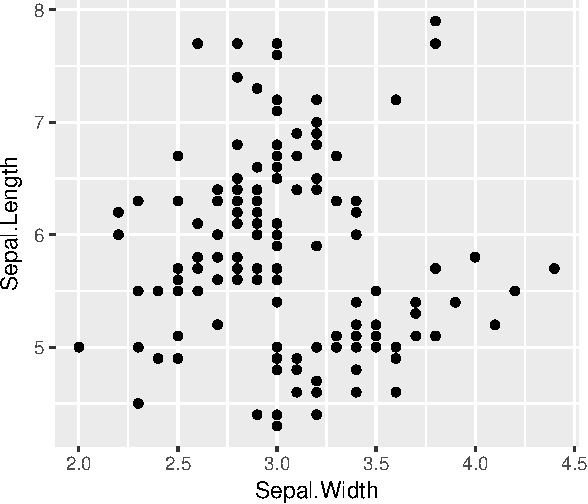
\includegraphics{6-datavis_files/figure-latex/ex1a-scatterplot-1.pdf}

\begin{enumerate}
\def\labelenumi{\alph{enumi}.}
\setcounter{enumi}{1}
\tightlist
\item
  Map \texttt{Species} to \texttt{colour} in \texttt{aes()}.
\end{enumerate}

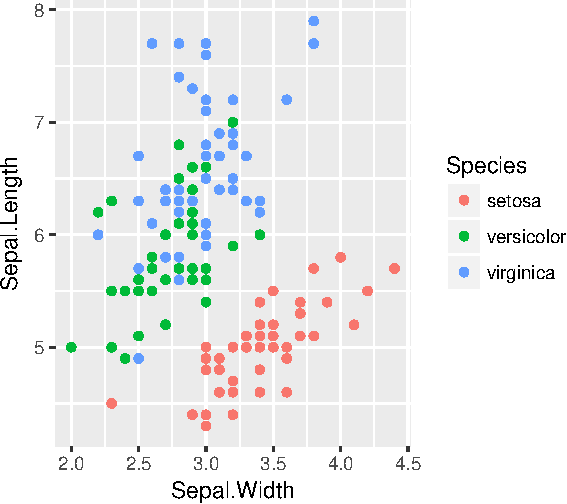
\includegraphics{6-datavis_files/figure-latex/ex1b-scatterplot-1.pdf}

\begin{enumerate}
\def\labelenumi{\alph{enumi}.}
\setcounter{enumi}{2}
\tightlist
\item
  Add the title to the plot:
  \texttt{"Scatterplot\ of\ Petal.Width\ and\ Petal.Length"} (use
  \texttt{ggtitle()} function).
\end{enumerate}

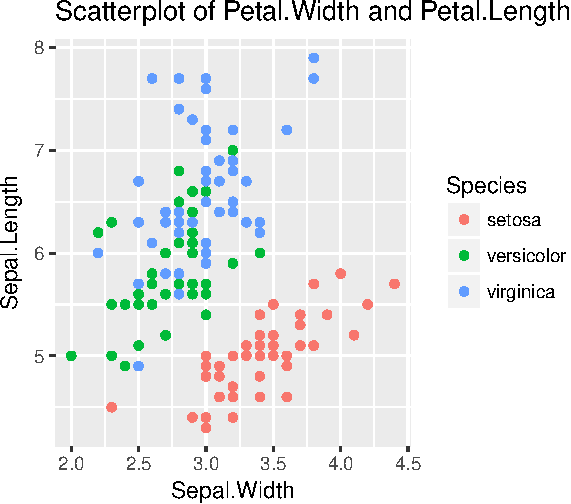
\includegraphics{6-datavis_files/figure-latex/ex1c-scatterplot-1.pdf}

\begin{enumerate}
\def\labelenumi{\alph{enumi}.}
\setcounter{enumi}{3}
\tightlist
\item
  Customize plot title by adding
  \texttt{theme(plot.title\ =\ element\_text())} to the plot and setting
  \texttt{colour} argument to \texttt{"red"}, \texttt{size} to 16 and
  \texttt{face} to \texttt{"bold"}.
\end{enumerate}

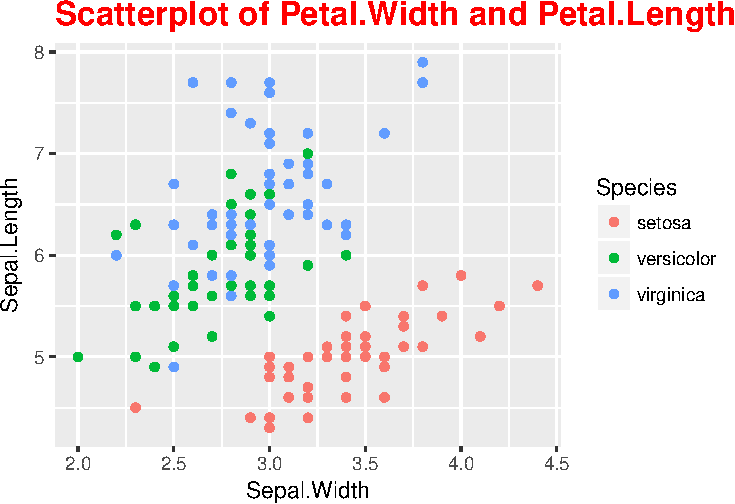
\includegraphics{6-datavis_files/figure-latex/ex1d-scatterplot-1.pdf}

\section{Barplot}\label{barplot}

\subsection{Exercise 1}\label{exercise-1-14}

Let us consider \texttt{mpg} dataset.

\begin{enumerate}
\def\labelenumi{\alph{enumi}.}
\tightlist
\item
  Represent graphically with a barplot the number of cars for each
  class.
\end{enumerate}

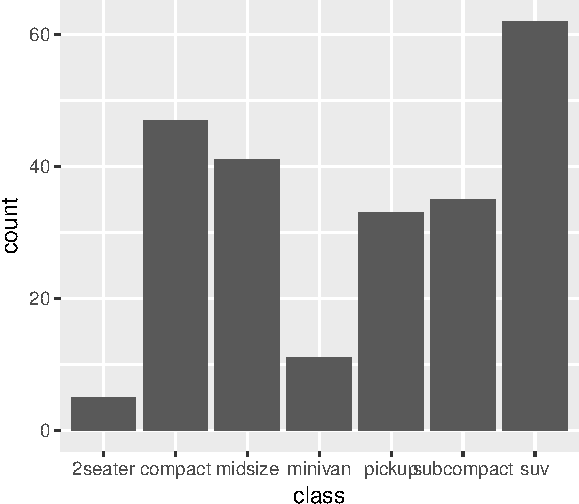
\includegraphics{6-datavis_files/figure-latex/ex2a-bargraph-1.pdf}

\begin{enumerate}
\def\labelenumi{\alph{enumi}.}
\setcounter{enumi}{1}
\tightlist
\item
  Represent graphically with a barplot, the distribution of manufacturer
  for each class (map \texttt{manufacturer} variable to \texttt{fill}).
\end{enumerate}

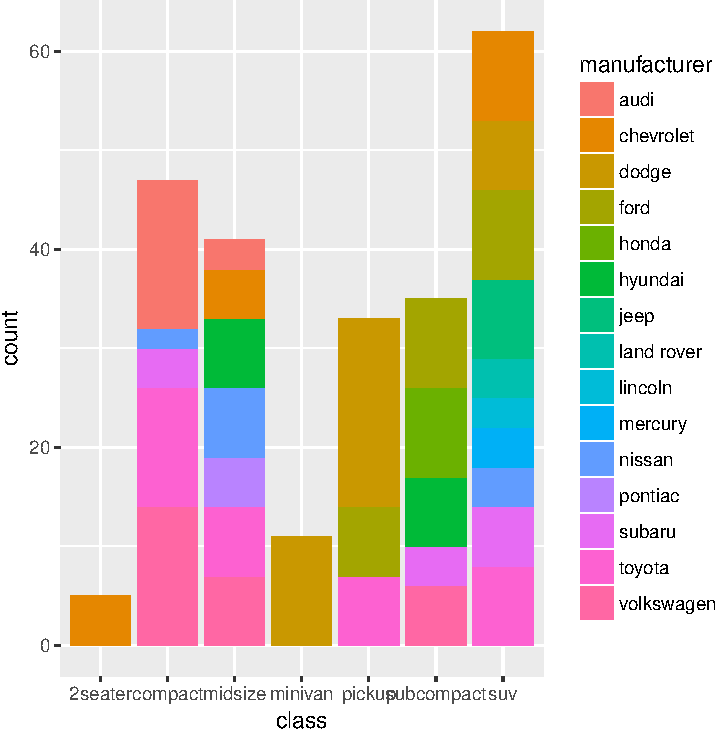
\includegraphics{6-datavis_files/figure-latex/ex2b-bargraph-1.pdf}

\clearpage

\section{Histogram}\label{histogram}

\subsection{Exercise 1}\label{exercise-1-15}

Let us consider \texttt{iris} dataset.

\begin{enumerate}
\def\labelenumi{\alph{enumi}.}
\tightlist
\item
  Represent the distribution of \texttt{Sepal\_Length} variable with an
  histogram.
\end{enumerate}

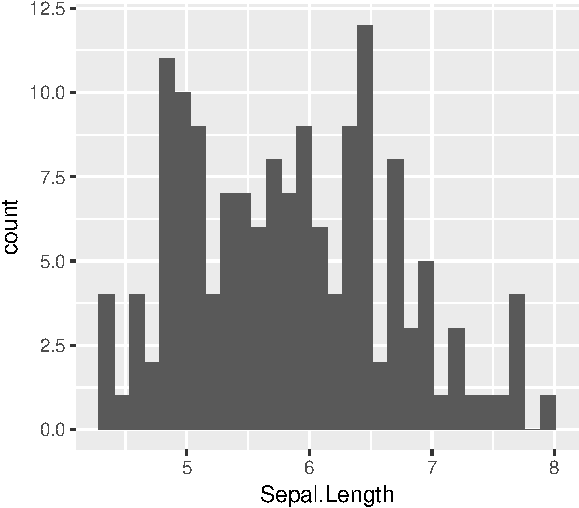
\includegraphics{6-datavis_files/figure-latex/ex3a-histogram-1.pdf}

\begin{enumerate}
\def\labelenumi{\alph{enumi}.}
\setcounter{enumi}{1}
\tightlist
\item
  Represent each level of \texttt{Species} variable in a different
  panel. Use \texttt{facet\_grid()} function.
\end{enumerate}

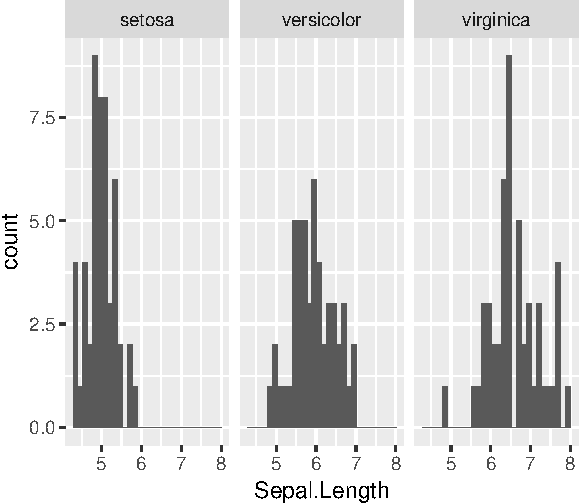
\includegraphics{6-datavis_files/figure-latex/ex3b-histogram-1.pdf}

\clearpage

\section{Boxplot}\label{boxplot}

\subsection{Exercise 1}\label{exercise-1-16}

Let us consider \texttt{iris} dataset.

\begin{enumerate}
\def\labelenumi{\alph{enumi}.}
\tightlist
\item
  Build a boxplot to compare the differences of sepal width accordingly
  to the type of iris species.
\end{enumerate}

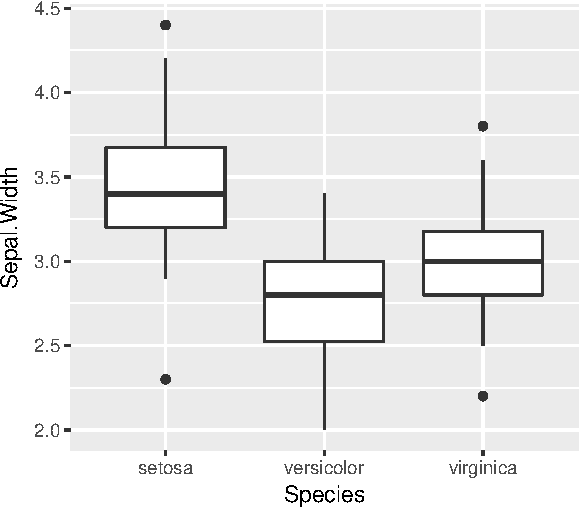
\includegraphics{6-datavis_files/figure-latex/ex4a-boxplot-1.pdf}

\begin{enumerate}
\def\labelenumi{\alph{enumi}.}
\setcounter{enumi}{1}
\tightlist
\item
  Set the fill colour of boxes as \texttt{"\#00FFFF"}, the lines colour
  of boxes as \texttt{"\#0000FF"} and the outliers colour as
  \texttt{"red"}.
\end{enumerate}

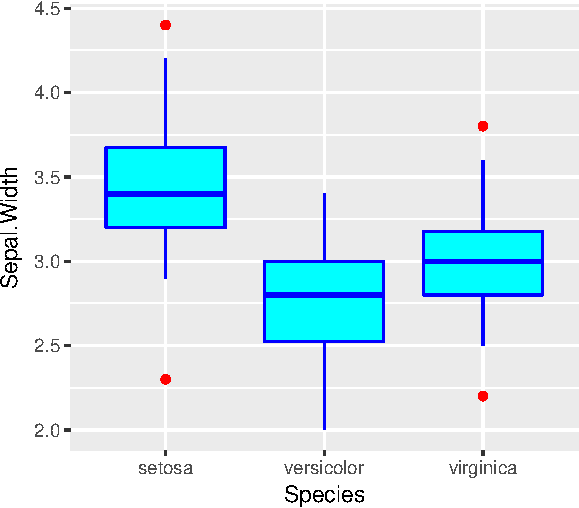
\includegraphics{6-datavis_files/figure-latex/ex4b-boxplot-1.pdf}

\begin{enumerate}
\def\labelenumi{\alph{enumi}.}
\setcounter{enumi}{2}
\tightlist
\item
  Add the plot title: \texttt{"Boxplot\ of\ Sepal.Width\ vs\ Species"}.
\end{enumerate}

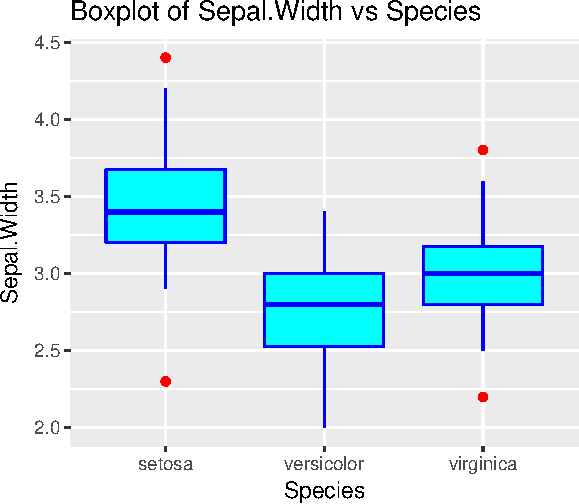
\includegraphics{6-datavis_files/figure-latex/ex4c-boxplot-1.pdf}

\clearpage

\section{Lineplot}\label{lineplot}

\subsection{Exercise 1}\label{exercise-1-17}

Let us suppose that the observations on \texttt{iris} are taken along
time.\\
So let us consider the following dataset, named \texttt{iris2}, in which
\texttt{time} variable is added:

\begin{Shaded}
\begin{Highlighting}[]
\KeywordTok{require}\NormalTok{(dplyr)}
\NormalTok{iris2 <-}\StringTok{ }\NormalTok{iris %>%}\StringTok{ }\KeywordTok{mutate}\NormalTok{(}\DataTypeTok{time=}\DecValTok{1}\NormalTok{:}\DecValTok{150}\NormalTok{)}
\end{Highlighting}
\end{Shaded}

\begin{enumerate}
\def\labelenumi{\alph{enumi}.}
\tightlist
\item
  Build a lineplot to visualize the measures of \texttt{Sepal.Length}
  variable along time.
\end{enumerate}

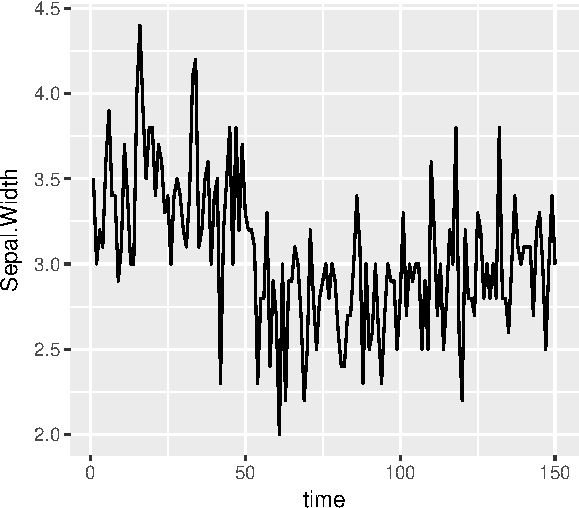
\includegraphics{6-datavis_files/figure-latex/ex5b-lineplot-1.pdf}

\chapter{Statistical models}\label{statistical-models}

Before starting the exercises, load the following libraries, supposing
they are already installed.

\begin{Shaded}
\begin{Highlighting}[]
\KeywordTok{require}\NormalTok{(dplyr)}
\KeywordTok{require}\NormalTok{(ggplot2)}
\KeywordTok{require}\NormalTok{(qdata)}
\end{Highlighting}
\end{Shaded}

\section{Linear Models}\label{linear-models}

\subsection{Exercise 1}\label{exercise-1-18}

The number of impurities (lumps) present in the containers of paint
depends on the rate of agitation applied to the container. A researcher
wants to determine the relation between the rate of agitation and the
number of lumps, so he conducts an experiment. He applies different
rates of agitation (\texttt{Stirrate}) to 12 containers of paint and he
counts the number of impurities (lumps) present in the containers of
paint (\texttt{Impurity}).

\begin{Shaded}
\begin{Highlighting}[]
\KeywordTok{data}\NormalTok{(paint)}
\KeywordTok{head}\NormalTok{(paint)}
\end{Highlighting}
\end{Shaded}

\begin{verbatim}
## # A tibble: 6 × 2
##   Stirrate Impurity
##      <int>    <dbl>
## 1       20      8.4
## 2       38     16.5
## 3       36     16.4
## 4       40     18.9
## 5       42     18.5
## 6       26     10.4
\end{verbatim}

\begin{enumerate}
\def\labelenumi{\alph{enumi}.}
\item
  Let us compute the main descriptive statistics of \texttt{Impurity}.
\item
  Let us graphically represent the relation between \texttt{Impurity}
  and \texttt{Stirrate} variables (add regression line to the
  scatterplot).
\item
  Let us compute a simple linear regression between \texttt{Impurity}
  and \texttt{Stirrate}.
\item
  Does \texttt{Stirrate} influence \texttt{Impurity}? How? Let us
  analyze the model fitted by using \texttt{summary()} function.
\item
  Let us check (final) models residuals.
\end{enumerate}

\subsection{Exercise 2}\label{exercise-2-8}

A pressure switch has a membrane whose thickness (in mm) influences the
pressure required to trigger the switch itself. The aim is to determine
the thickness of the membrane for which the switch ``trig'' with a
pressure equal to 165 ± 15 KPa. 25 switches with different thickness
(\texttt{DThickness}) of the membrane was analysed, measuring the
pressure at which each switch opens (KPa) (\texttt{SetPoint}).

\begin{Shaded}
\begin{Highlighting}[]
\KeywordTok{data}\NormalTok{(switcht)}
\KeywordTok{head}\NormalTok{(switcht)}
\end{Highlighting}
\end{Shaded}

\begin{verbatim}
## # A tibble: 6 × 2
##   DThickness SetPoint
##        <dbl>    <dbl>
## 1        0.9  223.523
## 2        0.6  157.131
## 3        0.5  149.307
## 4        0.8  200.146
## 5        0.8  199.974
## 6        0.7  166.919
\end{verbatim}

\begin{enumerate}
\def\labelenumi{\alph{enumi}.}
\item
  Let us compute the descriptive statistics of \texttt{SetPoint}
  variable.
\item
  Let us graphically represent the relation between \texttt{DThickness}
  and \texttt{SetPoint}(add regression line to the graph).
\item
  Let us compute a linear regression between \texttt{DThickness} and
  \texttt{SetPoint} and check the residuals of the fitted model.
\item
  Does \texttt{DThickness} influences \texttt{SetPoint}? Let us analyze
  the model fitted by using \texttt{summary()} function.
\item
  Let us check (final) models residuals.
\end{enumerate}

\chapter{Data Mining}\label{data-mining}

Before starting the exercises, load the following libraries, supposing
they are already installed.

\begin{Shaded}
\begin{Highlighting}[]
\KeywordTok{require}\NormalTok{(qdata)}
\KeywordTok{require}\NormalTok{(dplyr)}
\KeywordTok{require}\NormalTok{(ggplot2)}
\KeywordTok{require}\NormalTok{(nnet)}
\end{Highlighting}
\end{Shaded}

\section{Neural Networks}\label{neural-networks}

\subsection{Exercise 1}\label{exercise-1-19}

Consider \texttt{iris} dataset.

\begin{Shaded}
\begin{Highlighting}[]
\KeywordTok{data}\NormalTok{(iris)}
\KeywordTok{head}\NormalTok{(iris)}
\end{Highlighting}
\end{Shaded}

\begin{verbatim}
##   Sepal.Length Sepal.Width Petal.Length Petal.Width Species
## 1          5.1         3.5          1.4         0.2  setosa
## 2          4.9         3.0          1.4         0.2  setosa
## 3          4.7         3.2          1.3         0.2  setosa
## 4          4.6         3.1          1.5         0.2  setosa
## 5          5.0         3.6          1.4         0.2  setosa
## 6          5.4         3.9          1.7         0.4  setosa
\end{verbatim}

A botanist wants to to find a prediction model to assess the probability
of belonging to a specific species, for each flower, based on its sepal
and petal features.

\begin{enumerate}
\def\labelenumi{\alph{enumi}.}
\item
  Analyze the relationship between \texttt{Species} and the other
  variables of \texttt{iris} dataset. The following lines of code
  produces a scatterplot of \texttt{Sepal.Length} and
  \texttt{Sepal.Width} by \texttt{Species}.

\begin{Shaded}
\begin{Highlighting}[]
\KeywordTok{ggplot}\NormalTok{(}\DataTypeTok{data=}\NormalTok{iris, }\DataTypeTok{mapping=}\KeywordTok{aes} \NormalTok{(}\DataTypeTok{x=}\NormalTok{Sepal.Length, }\DataTypeTok{y=}\NormalTok{Sepal.Width, }\DataTypeTok{colour=}\NormalTok{Species)) +}
\StringTok{  }\KeywordTok{geom_point}\NormalTok{()}
\end{Highlighting}
\end{Shaded}

  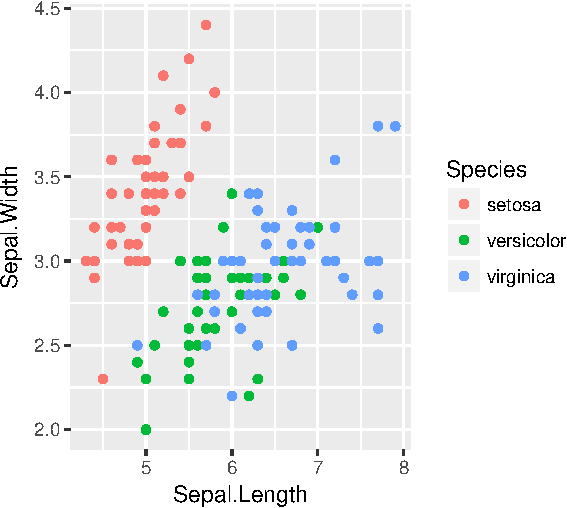
\includegraphics{8-datamin_files/figure-latex/scatterplot_1-1.pdf}

  Generate a scatterplot to analyze the relationship between
  \texttt{Petal.Length} and \texttt{Petal.Width} by \texttt{Species}.
  Comment the results.
\item
  Divide the dataset in train and test dataset in this way:

\begin{Shaded}
\begin{Highlighting}[]
\KeywordTok{set.seed}\NormalTok{(}\DecValTok{1}\NormalTok{)}
\NormalTok{samp <-}\StringTok{ }\KeywordTok{c}\NormalTok{(}\KeywordTok{sample}\NormalTok{(}\DecValTok{1}\NormalTok{:}\DecValTok{50}\NormalTok{,}\DecValTok{25}\NormalTok{), }\KeywordTok{sample}\NormalTok{(}\DecValTok{51}\NormalTok{:}\DecValTok{100}\NormalTok{,}\DecValTok{25}\NormalTok{), }\KeywordTok{sample}\NormalTok{(}\DecValTok{101}\NormalTok{:}\DecValTok{150}\NormalTok{,}\DecValTok{25}\NormalTok{))}
\NormalTok{train <-}\StringTok{ }\NormalTok{iris[samp,] }
\NormalTok{test <-}\StringTok{ }\NormalTok{iris[-samp,]  }
\end{Highlighting}
\end{Shaded}

  and estimate a Neural Network model on train sample to assess the
  probability of belonging to a specific species, for each flower, based
  on its measures of \texttt{Sepal.Length}, \texttt{Sepal.Width},
  \texttt{Petal.Length}, and \texttt{Petal.Width}. Use \texttt{nnet()}
  function and set the \texttt{size} (number of units in the hidden
  layer) to 2.
\item
  Use \texttt{predict()} function to gain the predictions on test
  sample. Add \texttt{type\ =\ "class"} argument to \texttt{predict()}
  function. Add the prediction estimated to \texttt{test} dataset.
\item
  Built a frequency table to compare the original distribution of
  \texttt{Species} and that predicted in \texttt{test} data. Comment the
  results.
\end{enumerate}


\end{document}
